\documentclass[a4paper,11pt]{scrreprt}                       % default is A4 paper style and 11pt font size


%%%%%%%%%%%% version history %%%%%%%%%%%%%%%%%%%%%%%%%%%%%%%%%%%
%27.05.2021: updates about layout/plagiarism from Monica Patrascu, Bogdan Dumitrescu
%25.04.2020:  modified the lst definitions (monospaced, gray); localized versions (romanian) for the \autoref command; updated the romanian.lbx file
%26.03.2017:    corrections for the latex source-code: diacritics issues; corrected the glossaries and added listings packages; added fontspec (only works with xelatex/lualatex !!!)
%2014:          put in latex version + some small additions - Florin Stoican
%2013:          content from Dan Stefanoiu
%%%%%%%%%%%%%%%%%%%%%%%%%%%%%%%%%%%%%%%%%%%%%%%%%%%%%%%%%%%%%%%%%%%%%%%%%


%%%%%%%%%%%% macros for various paths %%%%%%%%%%%%%%%%%%%%%%%%%%%%%%%%%%%
\def \cls {./cls} 																					 % path to common latex files (change for your own relative/absolute path)
\def \pics {./pics}      																		 % path to pics files (change for your own relative/absolute path)
\def \chapters {./chapters}      														 % path to chapter files (change for your own relative/absolute path)
\def \code {./code}      													        	 % path to source code files (change for your own relative/absolute path)

% you don't have to use them but it's nicer this way
%%%%%%%%%%%%%%%%%%%%%%%%%%%%%%%%%%%%%%%%%%%%%%%%%%%%%%%%%%%%%%%%%%%%%%%%%

% language={english/romanian} selects between the languages used in the manusript (changes, e.g., the name of the chapter)
% type={bachelor/master/phd} selects between the type of manusript (changes, e.g., the titlepage make-up)
\usepackage[language=romanian,type=bachelor]{\cls/standard} % introduces useful packages and commands(CHANGE ONLY IF YOU KNOW WHAT YOU'RE DOING)
\addbibresource{\cls/bib.bib}																% bib resource (using biblatex package, for complex stuff use the biber backend instead of bibtex
\newglossaryentry{computer}
{
  name=computer,
  description={is a programmable machine that receives input,
               stores and manipulates data, and provides
               output in a useful format}
}

\newacronym[longplural={Frames per Second}]{fpsLabel}{FPS}{Frame per Second}
\newacronym{lvm}{LVM}{Logical Volume Manager}        																	% put here all your glossary terms; only the ones actually used will appear in the glossary list of the manuscript

\begin{document}

%%%%%%%%%%%%%%%%%%%%%%% frontmatter %%%%%%%%%%%%%%%%%%%%%%%%%%%%%%%%%%%%%
\pagenumbering{roman}																				% default numbering for the frontmatter is roman

\title{Titlu lucrare de diplomă}					    % title of your manuscript
\author{nume student}																				% author name
\advisor{nume coordonator}																			    % advisor name

\maketitle

% show table of contents, figures, tables and algorithms

\tableofcontents 
\printnoidxglossaries																				% \printglossaries works only if the makeindex has the correct arguments
\listoffigures 
\addcontentsline{toc}{chapter}{\listfigurename}
\listoftables
\addcontentsline{toc}{chapter}{\listtablename}
\listofalgorithmes
\addcontentsline{toc}{chapter}{\listalgorithmcfname}

\clearpage

%%%%%%%%%%%%%%%%%%%%%%% mainmatter %%%%%%%%%%%%%%%%%%%%%%%%%%%%%%%%%%%%%%
\pagenumbering{arabic}																			% default numbering for the mainmatter is arabic

% here is the text of you manuscript; you can put it directly here but it is better to include files (the main file will be more compact)
\chapter{Indicații de redactare}
\label{chap:intro}

\myLettrine{L}{ucrarea} de diplomă este subiectul examenului de finalizare a studiilor și trebuie să reflecte contribuţiile personale ale autorului, i.e. studentul candidat. Lucrarea de diplomă descrie un proiect realizat de autor sub îndrumarea cadrului didactic ales, de obicei, la începutul anului terminal al studiilor de licență. Examenul de finalizare al studiilor se desfășoară conform procedurilor indicate la aviziere și prin website-ul facultăţii. Ghidul de față este valabil pentru studenții direcției B: Ingineria Sistemelor.

\textbf{Respectarea} acestui ghid este \textbf{obligatorie}.

\section{Conținutul lucrării de diplomă}

Lucrarea de diplomă trebuie să reflecte capacitatea autorului de a înțelege și utiliza conceptele din subdomeniul specific al proiectului ales, capacitatea acestuia de a sintetiza cunoștințele acumulate pe parcursul studiilor, și de a le prezenta într-o manieră riguroasă. Lucrarea va fi scrisă într-una din limbile română sau engleză, la alegerea autorului, după consultarea profesorului coordonator.

\textbf{Lucrarea de diplomă se redactează la persoana I singular, pentru a evidenția activitățile autorului} vs. contribuţiile altor cercetători în domeniu ce stau la baza proiectului.

Spre exemplu, ``\emph{Pentru proiectarea algoritmului de reglare, am ales inițial o metodă în frecvență}.'' se referă la contribuția proprie a autorului, în timp ce ``\emph{Pentru proiectarea algoritmului de reglare s-a ales inițial o metodă în frecvență (Popescu, 2000)}.'' reflectă contribuția lucrării citate prin (Popescu, 2000) la subiect.


Lucrarea de diplomă are între 30 şi 40 de pagini. În aceste pagini nu se numără pagina de titlu, cuprinsul, anexele, bibliografia și lista contribuţiilor personale.

Lucrarea de diplomă este compusă din:

\begin{enumerate}[label=\alph*.]
	\item Pagină de titlu
	\item Cuprins
	\item Introducere
	\item Capitole - corpul lucrării
	\item Concluzii
	\item Anexe (dacă este cazul)
	\item Bibliografie  
	\item Lista contribuțiilor personale
\end{enumerate}
La alegere, se pot include liste ale figurilor, tabelelor și algoritmilor.

\section{Introducere și concluzii}

Capitolul introductiv al lucrării de diplomă are o lungime de 1-2 pagini, cuprinzând scopul și obiectivele lucrării. La alegere, se poate include și motivația alegerii temei. Se recomandă descrierea cât mai clară a obiectivelor lucrării.

Concluziile lucrării rezumă îndeplinirea obiectivelor lucrării prin prisma activității desfășurate pe parcusul realizării proiectului. Acestea conțin opiniile proprii ale autorului, susținute de rezultatele prezentate în corpul lucrării. Capitolul concluziilor nu este, de obicei, mai lung de 1 pagină.

\section{Corpul lucrării}

Structura capitolelor asociate corpului lucrării este la alegerea autorului, cu ilustrarea următoarelor componente: formularea problemei, soluția abordată, implementare (software și/sau hardware), rezultate / exemplu numeric.

Corpul lucrării de diplomă trebuie să conțină în principal contribuţiile autorului, urmând pașii logici de proiectare conform temei alese.

\textbf{Elementele așa-zise ``teoretice'' ce reflectă cunoștințe din domeniu deja cunoscute trebuie să nu depășească 1/3 din corpul lucrării. Se recomandă includerea exclusivă a acelor componente absolut necesare pentru prezentarea contribuțiilor proprii.} Spre exemplu, în cazul proiectării unui sistem de conducere, este necesară menționarea indicatorilor de performanță ce vor fi utilizați pentru validarea sistemului; în schimb, nu este necesară includerea testului de stabilitate Hurwitz, ci numai aplicarea acestuia în contextul studiat.

\textbf{Schemele și structurile specifice proiectului (fie ele din domeniul reglării, al proiectării hardware, sau al sistemelor software) trebuie sa se limiteze numai la cele ce țin strict de tema și subiectul lucrării.} Spre exemplu, în cazul proiectării unei aplicații pentru reglarea prin comandă wireless a unui proces, este relevantă schema structurii programului proiectat, însă nu este necesară descrierea în detaliu a protocolului de comunicație prin bluetooth. 

În cazurile în care tema lucrării de diplomă, la indicațiile îndrumătorului, continuă/completează/extinde rezultatele unei lucrări științifice existente, iar acestea sunt relativ noi sau nu se regăsesc în curicula uzuală a anilor de studiu, este permisă rezumarea, pe scurt, a acestora în scopul creșterii lizibilității lucrării.

\textbf{Este interzisă copierea formulelor, ecuațiilor, figurilor, imaginilor etc. din surse externe, inclusiv cursuri.} Toate aceste elemente incluse în lucrarea de diplomă trebuie să fie redactate / desenate de autor. Este absolut obligatorie citarea surselor acestor elemente. În cazul figurilor, se admite o singură excepție per lucrare, numai atunci când imaginea respectivă descrie un rezultat al altor cercetători (publicat întro
lucrare științifică citată).

\section{Anexe}

Anexele lucrării de diplomă conțin informație-suport care susține realizarea proiectului, cum ar fi: teoreme, formule de calcul uzuale, fișe tehnice pentru componente (senzori, plăci etc.), extrase de cod, scheme electrice, componente intermediare relevante din parcusul realizării proiectului, descriere IDE-uri, limbaje de programare, algoritmi clasici.

\section{Lista contribuţiilor personale}

Lista contribuţiilor personale este \textbf{obligatorie}. Aceasta este un tabel redactat pe 1 pagină inserată la finalul lucrării. Lista enumeră contribuțiile personale (de ex. documentare, implementare cod și/sau soluție hardware, testare, etc), probleme întâmpinate în proiectare, precum și durata de realizare a fiecărui element enumerate anterior. Acest tabel este echivalent cu borderoul caietului de laborator sau a jurnalului de activități (engl. \emph{log}) utilizat pe parcursul realizării proiectului.

Durata este exprimată în zile echivalente de lucru, adică 1 zi = 8 ore.

Tabelul \ref{tab:lista_contrib} arată forma recomandată de prezentare a contribuțiilor personale.

\begin{table}[ht!]
\begin{tabular}{|c|c|c|}
\hline
\multicolumn{3}{|c|}{\textbf{Titlu lucrare de diplomă}} \\
\multicolumn{3}{|c|}{\textbf{Nume autor}} \\
\multicolumn{3}{|c|}{\textbf{Nume coordonator/îndrumător}} \\
\hline
 & Activitate & Durată [zile] \\
\hline
1 & \hspace*{12cm} & \\
\hline
2 &  & \\
\hline
3 &  & \\
\hline
\end{tabular}
\centering
\caption{Lista contribuțiilor personale}
\label{tab:lista_contrib}
\end{table}

\section{Redactarea lucrării de diplomă}

\textbf{Lucrarea de diplomă nu este un manuscris, ci un produs finit, prezentarea acestuia necesitând un anumit grad de finisare în formatare.}

Formatul uzual al paginilor pentru redactarea lucrării de diplomă are următoarele caracteristici:

\begin{itemize}
\item pagină A4
\item 	margini de 2cm sus, jos \c si la dreapta
\item  margine de 3cm la stânga
\item spaţiere simplă, la un rând (\emph{single line})
\end{itemize}

\textbf{Acest document respectă formatul propus.}

Fonturile cele mai lizibile pentru redactarea lucrării de diplomă sunt acele
fonturi care au corpul literei de dimensiune echilibrată în lăţime şi înălţime. Exemple de fonturi care se pretează redactării lucrării de diplomă sunt: Times New Roman 12pt, Arial 12pt, Verdana 11pt, Adobe Caslon Pro12 pt, Linotype Palatino 12pt, Helvetica 12pt, Neutra Text 12pt, Kozuka Mincho 11pt.

Nu se vor utiliza fonturi de dimensiune mai mare decât 12pt în corpul lucrării, excepție făcând titlurile capitolelor. Se recomandă alegerea unui font care conţine diacritice, în cazul redactării lucrării în limba română.

Lucrarea de diplomă se redactează, în întregime, cu acelaşi font. Excepţie fac anexele, unde este posibilă utilizarea unui font special pentru transcrierea scripturilor şi a programelor, de exemplu: Courier şi/sau Courier New cu dimensiune de 10 sau 11pt.

Paragrafele se despart printr-un rând liber. Începutul unui paragraf se marchează prin deplasarea la dreapta a primului rând din paragraf, de obicei cu 1 sau 1.5 cm. Corpurile de text se distribuie pe orizontală de la un capăt al celuilalt al paginii (aliniere \emph{justified}), și nu la stânga. 

\subsection{Pagina de titlu} 
Pagina de titlu conţine numele lucrării de diplomă, numele autorului și al coordonatorului acestuia, numele universităţii/facultăţii/departamentului, orașul și anul în care a fost scrisă aceasta. Prima pagina a acestui document prezintă o sugestie de formatare a paginii de titlu pentru lucrările de diplomă.

\subsection{Cuprinsul lucrării de diplomă} 
Cuprinsul lucrării de diplomă conţine toate titlurile capitolelor, secţiunilor şi subsecţiunilor, în ordinea în care acestea apar în lucrare. Se recomandă să nu se prescurteze cuvintele "Capitol" şi "Secțiune" în cazul în care acestea sunt utilizate înainte de numărul capitolului şi al secţiunii sau subsecţiunii respective. Uzual, aceste cuvinte se omit.

\subsection{Numerotare}

Paginile lucrării se numerotează în ordine. Nu este indicată reînceperea numerotării paginilor cu fiecare capitol. De asemenea, nu este indicată numerotarea paginii de titlu.

Numerele de pagini se includ în câmpuri speciale de subsol (Footer), în care fontul utilizat trebuie să fie același cu restul lucrării și cu 1 sau 2 puncte tipografice mai mic. Optional, se poate include un câmp conţinând titlul lucrării în zona superioară a paginii (Header), acesta necesitând aceeași dimensiune de font adoptată pentru numerele de pagini.

\subsection{Figuri, grafice și tabele}

 Figurile și tabelele trebuie să aibă un titlu care să menţioneze tipul obiectului respectiv, conţinutul acestuia și numărul acestuia în cadrul capitolului:

\begin{description}
\item[Figura c.n.] desemnează o figură, c fiind identificatorul capitolului, iar n reprezentând numărul figurii în cadrul acelui capitol; acest titlu va fi urmat de numele figurii, descriind conţinutul acesteia. De exemplu: Figura 3.2. Sistem de reglare automată a presiunii va fi titlul figurii a doua din capitolul 3, conţinând structura unui sistem de reglare automată a presiunii. 
\item[Tabelul c.n.] desemnează un tabel, c fiind identificatorul capitolului, iar n reprezentând numărul tabelului în cadrul acelui capitol; acest titlu va fi urmat de numele tabelului, descriind conţinutul acestuia. De exemplu: Tabelul 5.6. Caracteristici tehnice ale traductorului de temperatură va fi titlul tabelului al șaselea din capitolul 5, conţinând caracteristicile tehnice ale unui traductor de temperatură.
\end{description}
Graficele sunt considerate figuri și vor purta titluri adecvate. Graficele trebuie să aibă o etichetă pe fiecare axă, descriind semnificaţia acesteia, menţionând unitatea de măsură acolo unde este cazul. De exemplu, pentru răspunsul în timp al unui sistem de ordinul I oarecare, este îndeajuns a atașa eticheta y pe ordonată și eticheta t pe abscisă. Însă dacă acest răspuns aparţine unui model al unui proces fizic, se va menţiona unitatea de măsură pe fiecare axă, de exemplu y[m] și t[s].

Pentru o tipărire corectă, toate figurile și graficele ar trebui salvate la o rezoluţie de cel putin 300dpi pentru cele color și 100dpi pentru cele alb-negru. Se recomandă salvarea acestora în format .tiff sau .png pentru conservarea calităţii imaginilor.

Se recomandă alinierea centrală a figurilor. Tabelele se pot alinia la stânga, lăsând faţă de marginea paginii (acolo unde este posibil si dacă tabelul nu acoperă toată lăţimea paginii) aceeași dimensiune ca și în cazul primului rând al paragrafelor.

\subsection{Ecuaţii}

	Ecuaţiile se scriu cu aceeași înălţime de font ca și corpul textului și se numerotează în ordinea apariţiei în text: (c.n) unde c reprezintă identificatorul capitolului curent, iar n este numărul ecuaţiei în capitol. Ecuaţiile pot avea eticheta de identificare la stânga sau la dreapta. Ecuaţiile se pot alinia centrat sau la stânga. De exemplu:

\be
\label{eq:test}
5+x=0
\ee
unde 1 reprezintă numărul capitolului, iar 1 este numărul ecuaţiei în cadrul acestuia. Înainte și după fiecare ecuaţie se lasă un rând liber.


\subsection{Bibliografie}

	Lista bibliografică este o componentă esenţială a lucrării de diplomă, aceasta demonstrând documentarea efectuată de către autor și marcând corespunzător ideile care nu îi aparţin acestuia. Bibliografia este formată dintr-o listă ordonată alfabetic. \textbf{Toate} elementele acestei liste trebuie \textbf{citate în text}.



\chapter{Despre plagiat}
\label{chap:div}


În România, legea drepturilor de autor este \textbf{Legea nr. 8/1996} completată de \textbf{Legea nr. 285 din 23 iunie 2004} şi \textbf{Ordonanţa de urgenţă 123 din 1 septembrie 2005}.

\myLettrine{C}{onform} Dicţionarului Explicativ al Limbii Române:

\blockquote{PLAGIA: A-şi însuşi, a copia total sau parţial ideile, operele etc. cuiva, prezentându-le drept creaţii personale; a comite un furt literar, artistic sau ştiinţific.}

În contextul lucrărilor ştiinţifice, plagiatul reprezintă utilizarea ideilor, tehnologiilor, rezultatelor sau textelor altor persoane, omițând referirea lucrării originale.

În cazul secţiunilor de text citate din alte opere (exemplu mai sus), se recomandă încadrarea între ghilimele a textului, cu mențiunea sursei. Nu se recomandă preluări de text mai lungi de 2-3 rânduri.

În cazul prezentării unor idei, teorii, fapte statistice etc., care nu ţin de cultura generală și sunt preluate din alte opere, se recomandă re-povestirea prin prisma înțelegerii proprii și citarea sursei în prima frază. De exemplu: {\em Algoritmul X a fost propus în [3] și constă în următoarea secvență de operații.}

Modul cel mai simplu de evitare a plagiatului este formularea personală a lucrării, cu menționarea surselor acolo unde este cazul. Parafrazarea cu schimbarea câtorva cuvinte nu este suficientă.

Toate lucrările de diplomă sunt supuse unei verificări antiplagiat cu un program specializat. Rezultatele verificării sunt interpretate de un cadru didactic. Nu se poate vorbi despre un procent admisibil de similaritate cu texte existente. Copierea a 2-3 paragrafe fără a cita sursa, chiar și cu modificarea unor cuvinte, poate duce la scăderea notei la lucrarea de diplomă. Copierea unor porțiuni mari de text, de ordinul paginilor, poate duce la neprimirea în examenul de diplomă și eventual chiar la pedepse mai aspre. Desigur, este mai gravă prezentarea ca rezultate personale a unor rezultate obținute de alții (deci copierea "contribuțiilor proprii") decât copierea unor "noțiuni teoretice", dar ambele sunt la fel de interzise.



\chapter{Detalii formatare \LaTeX}
\label{chap:main}

\myLettrine{M}{aterialul} curent folosește ca template clasa \textquote{scrrprt} la care s-au adăugat pachete și comenzi uzuale. 

\shadowbox{
\begin{minipage}{.95\textwidth}
Datorită folosirii pachetului \emph{fontspec} ce acceptă în mod nativ diacritice, fișierul sursă latex se poate compila doar cu \textbf{xelatex}, nu și cu \textbf{pdflatex}.
\end{minipage}
}

Pentru a păstra o structură cât mai compactă fișierele sursă s-au împărțit în următoarele categorii\footnote{Nu este obligatoriu să se păstreze aceeași structură dar este recomandat, pentru a păstra o formatare compactă.}:
\begin{description}[style=nextline]
\item[thesis.tex] reprezintă fișierul \textquote{main} în care toate celelalte fișiere sunt apelate
\item[standard.sty] conține pachetele și comenzile folosite uzual
\item[bib.bib] conține câteva referințe în format \emph{bibtex}; referințe adiționale pot fi adăugate după necesități \url{https://texblog.org/2014/04/22/using-google-scholar-to-download-bibtex-citations/}
\item[upb-authoryear.bbx, upb-authoryear.cbx si romanian.lbx] definesc stilul bibliografic asociat intrărilor din lista bibliografică
\item[gls.tex] conține termeni de glosar ce pot fi adăugați la o \textquote{Listă de termeni} dacă se consideră necesar
\end{description}
Comentarii și scurte explicații (în engleză) referitor la rolul pachetelor și comenzilor se regasesc în aceste fișiere sursă.

Adițional, următoarea structură de dosare a fost folosită:
\begin{description}[style=nextline]
\item[cls] pentru stocarea fișierelor-sursă auxiliare (pentru introducerea de pachete/referințe bibliografice, etc.)
\item[pics] pentru stocarea imaginilor ce vor fi adaugate în manuscris
\item[chapters] pentru stocarea fișierelor \textquote{capitol} (pentru ușurința în lucru, am presupus că textul fiecărui capitol va fi pus într-un fișier sursă de sine-stătător)
\item[code] pentru stocarea fișierelor \textquote{sursă} ce vor fi apoi adăugate în manuscris
\end{description}

\begin{rem}
\label{rem:at}
În cazul în care se dorește modificarea structurii mai sus-menționate, o atenție sporită trebuie acordată referințelor făcute în cadrul fișierelor. \eor
\end{rem}

Fișierele au fost compilate folosind distribuția Miktex 2.9 (\url{http://miktex.org/2.9/setup}), cu ajutorul editorului de text TexnicCenter (\url{http://www.texniccenter.org/}). Detalii generale despre \LaTeX se pot găsi de exemplu în \url{http://tobi.oetiker.ch/lshort/lshort.pdf}. În cele ce urmează sunt prezentate câteva situații tipice.


\section{Exemple comenzi de tip float}
În această secțiune  vor fi exemplificate câteva construcții de tip \textquote{float}. În general, fiecărui float i se poate asocia un element de tip \emph{legendă} pentru a putea da o explicație detaliată și un element de tip \emph{etichetă}, ce va permite referirea la acest float în cadrul manuscrisului cât și enumerarea sa în cadrul listei asociate (de exemplu in \emph{lista de figuri} vor apare toate figurile definite în manuscris).

\subsection{Tabele}
Informații suplimentare despre tabele pot fi gâsite de exemplu în \url{http://en.wikibooks.org/wiki/LaTeX/Tables}.
Câteva exemple simple sunt ilustrate în continuare.

\begin{table}[ht!]
\begin{tabular}{llll}
\hline
Fault & Fault & Symbol & Type\\ 
No. & & & \\
\hline
1 & Sensor Fault & $\Delta\beta_{1,m1}$ & Fixed Value\\
2 & Sensor Fault & $\Delta\beta_{2,m2}$ & Gain Factor\\
3 & Sensor Fault & $\Delta\beta_{3,m1}$ & Fixed Value\\
4 & Sensor Fault & $\Delta\omega_{r,m1}$ & Fixed Value\\
5 & Sensor Fault & $\Delta\omega_{r,m2}$, $\Delta\omega_{g,m2}$ & Gain Factor\\ 
\hline
\end{tabular}
\centering
\caption{Faults affecting the wind turbine model}%Considered Faults}
\label{tab:faults}
\end{table}

\begin{table}[ht!]
\begin{center}
\begin{tabular}{|c|c|c|c|c|c|c|c|}
\hline
no. of hyperplanes&5&10&15&20&25&50&100\\ \hline
classical&9.91&64.06&91.74&511.47&306.04&$\cdots$&$\cdots$\\ \hline
enhanced&1.14&0.81&0.59&4.84&4.18&3.66&2.94\\ \hline
\end{tabular}
\end{center}
\caption{Numerical values for the solving of an MI optimization problem under classical and anhanced methods.}
\label{tab:run}
\end{table}

Atât \tabref{tab:faults} cât și \tabref{tab:run} vor aparea în lista de tabele și vor putea fi referite în text cu ajutorul etichetei asociate fiecăruia.

\subsection{Figuri}
În mod similar se pot afișa diverse imagini (se recomandă fie imagini în format raster de rezoluție suficientă, fie imagini in format vectorial -- eps, pdf, tikz). Detalii suplimentare se pot găsi de exemplu în \url{http://en.wikibooks.org/wiki/LaTeX/Floats,_Figures_and_Captions}.

\begin{figure}[!ht]
\begin{center}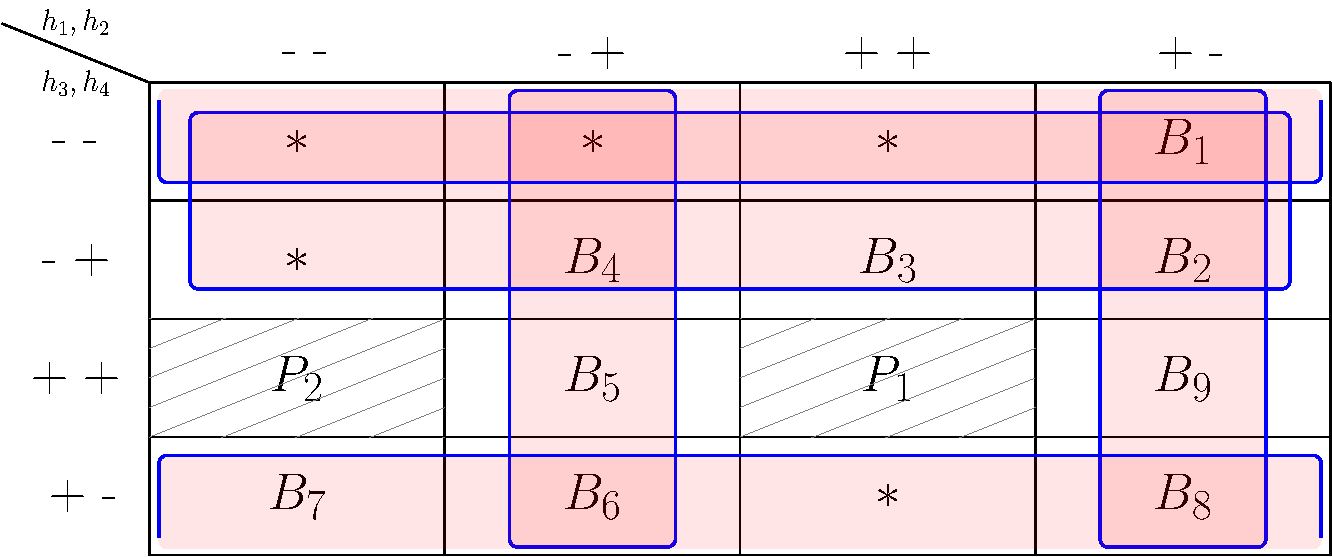
\includegraphics[width=\singlefigure]{\pics/binary/KarnaughDiagramForHyperplaneArrangement}\end{center}
	\caption{Karnaugh diagram for obaining the reduced cell representation}
	\label{fig:karnaugh}
\end{figure}

În \figref{fig:karnaugh} se ilustrează un exemplu simplu (o singură figură) iar în \figref{fig:int} se face uz de pachetul \textquote{subfig} ce permite o structură de tip tabel cu mai multe sub-figuri (fiecare dintre acestea poate fi referită în mod independent -- de exemplu, \figref{fig:int}\subref{fig:intc}).

\begin{figure}[!ht]
\begin{center}
  \subfloat[cut for each tuple]{\label{fig:inta}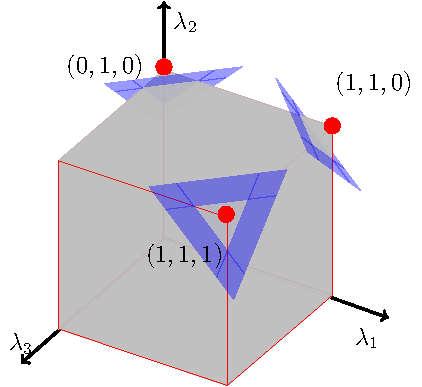
\includegraphics[width=\triplefigure]{\pics/binary/cutForEveryTuple}}
	\subfloat[cut for each complete face]{\label{fig:intb}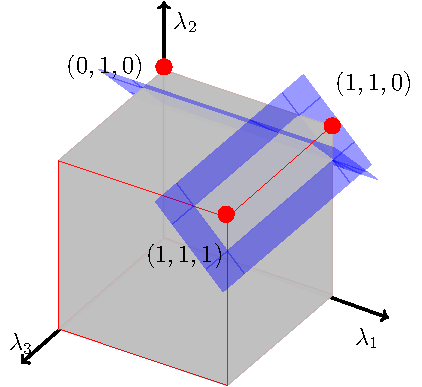
\includegraphics[width=\triplefigure]{\pics/binary/cutForEveryEdge}}
	\subfloat[only one cut]{\label{fig:intc}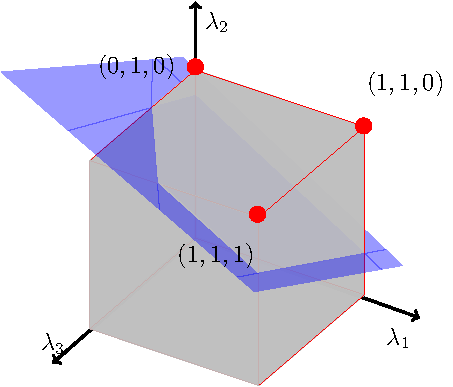
\includegraphics[width=\triplefigure]{\pics/binary/cutForAllTuples}}
	\caption{Exemplification of separating hyperplanes techniques}
	\label{fig:int}
\end{center}
\end{figure}


\begin{rem}
Dimensiunea unei figuri este determinată de argumentul opțional `width'. S-a preferat folosirea de macro-uri (\verb+\singlefigure+ și \verb+\triplefigure+) și nu valori \textquote{hard-coded} datorita flexibilității lor. Shimbând în preambul (în \emph{standard.sty}) valoarea unui astfel de macro se vor schimba automat dimensiunile figurilor ce îl folosesc, fără a mai fi nevoie să se modifice fiecare în parte. \eor
\end{rem}

\subsection{Algoritmi}

În exemplul de mai jos, \algref{alg:run} folosește pachetul \textquote{algorithm2e} pentru redactarea unui algoritm. Prin modificarea opțiunilor din preambulul documentului (în \emph{standard.sty}) este posibilă modificarea structurii/introducerea de noi cuvinte cheie/etc.

\begin{algorithm2e}
\caption{Fault tolerant scheme}
\label{alg:run}
\KwIn{$\mathcal{I}=\mathcal{I}_H(0)\cup \mathcal{I}_F(0);\quad\mathcal{I}_H(0)\neq \emptyset$}
$k \leftarrow$ the current sampling time\;
\ForEach{sensor $i\in \mathcal{I}_F(k-1)$}{
	\If{$r_i(k-1)\in R_i^F$ and $r_i(k) \in R_i^H$}{compute a timer $\bar \theta_i$ \;}
	}
\end{algorithm2e}

\section{Lista bibliografică}

Lista bibliografică este extrasă dintr-un fișier \textquote{*.bib} în care sunt stocate articole/cărți/conferințe în format bibtex (detalii suplimentare pot fi gasite la \url{http://en.wikibooks.org/wiki/LaTeX/Bibliography_Management}). Un exemplu al unei astfel de intrări este:


\begin{verbatim}
@article{gilbert1991linear,
 title={{Linear systems with state and control constraints: the theory and application of maximal output admissible sets}},
 author={Gilbert, EG and Tan, KT},
 journal={IEEE Transactions on Automatic Control},
 volume={36},
 number={9},
 pages={1008--1020},
 year={1991}
}
\end{verbatim}

Pentru citarea în text și listarea intrărilor citate în lista bibliografică s-a folosit pachetul \textquote{biblatex}. În cadrul acestui pachet, cele mai uzuale comenzi de citare sunt următoarele:
\begin{description}[style=nextline]
\item[citare simplă] \verb+\cite{...}+: \cite{bitsoris2006invariance}
\item[citare pusă între paranteze] \verb+\parencite{...}+: \parencite{gilbert1991linear}
\item[citare cu anul pus între paranteze] \verb+\textcite{...}+: \textcite{loechner1999polylib}
\item[citare cu intrări multiple] \verb+\cite{..., ..., ...}+: \cite{bellingham2002receding,garey1979computers,vitus_tunnel-milp:_2008,camponogara2002distributed}
\end{description}

În mod automat, intrările citate în text (și doar ele) vor fi puse în lista de referințe de la sfârșitul manuscrisului.


\section{Localizare: română versus engleză}

În fișierul principal (\emph{thesis.tex}), prin selectarea opțiunii \emph{language=english}, \emph{language=romanian} se poate alterna, respectiv, între formatarea în engleză și cea în română a textului. Câteva exemple sunt:
\begin{itemize}
\item numele cuprins-ului va alterna între \textquote{contents/cuprins}
\item în interiorul listei bibliografice caracterele de legatură se vor adapta (de exemplu, `and' devine `și')
\item \textquote{ghilimelele} se vor adapta la limba folosită (daca pentru a cita un fragment de text folosiți comenzile \verb+\textquote+ sau \verb+\blockquote+)
\item blocurile matematice își vor schimba eticheta, de exemplu `Theorem' devine `Teorema' 
\item referința la un element, de exemplu `Figure 2.3' devine `Figura 2.3'
\end{itemize}

Pentru diacritice (\u a,\^ a,\^ i, \c s, \c t etc.) se poate recurge fie la o codare explicită (\verb+\u a+, \verb+\^ a+, \verb+\^ i+, \verb+\c s+, \verb+\c t+) așa cum e detaliat în \url{http://en.wikibooks.org/wiki/LaTeX/Special_Characters} fie la scrierea lor direct de la o tastatura setată în limba romana într-un editor de text ce suportă utf8.


\section{Diverse}

\begin{description}[style=nextline]
\item[blocuri matematice] pentru blocurile tipic întălnite în matematică (Teoremă, Propoziție, Definiție, Remarcă, etc.) există definiții în preambul ce permit notarea/etichetarea și apelarea lor în mod automat. Spre exemplu, un bloc de tip teoremă se scrie astfel:

\begin{thm}
\label{thm:test}
Conținut teoremă ... urmat de simbolul de terminare a textului. \eot
\end{thm}
\begin{proof}
Demonstrație a afirmațiilor făcute în teoremă.
\end{proof}
Teorema poate fi apoi referită în text prin intermediul etichetei sale: \thmref{thm:test}.
\item[referințe în text]
Cu ajutorul etichetelor asociate blocurilor definite în latex, este posibilă referirea în mod automat a acestor elemente oriunde în manuscris. Prin adaugarea pachetului \emph{hyperref} aceste referințe devin link-uri ce fac legătura cu elementul față de care sunt asociate.
 
Exemple de referințe pot fi ecuații (\eqref{eq:test}), elemente de structură (\chapref{chap:intro}), blocuri matematice (\remref{rem:at}) sau figuri/tabele/algoritmi. Pentru multe dintre acestea,  în fișierele sursă s-au definit macro-uri. Deși nu este obligatoriu, recomandăm uzul acestora datorita flexibilității lor. De exemplu, folosind \verb+\figref{eticheta}+ putem să ne adaptam în mod automat la schimbarea limbajului de lucru (în preambul, acest macro va schimba, în funcție de opțiunea aleasă, între `Figure' și `Figura').

\item[termeni de glosar, acronime]
În fișierul \emph{./cls/gls.tex} introduceți termeni de glosar. Aceștia pot fi apoi folosiți prin apelarea comenzii \verb+\gls{numeTermen}+. Spre exemplu \gls{computer} este un termen de glosar iar \gls{fpsLabel} și \gls{lvm} sunt acronime (atunci când sunt apelate prima oară apar în forma desfășurată, la următorele apelări apar doar cu abreviere: \gls{fpsLabel} și \gls{lvm}). Acești termeni vor fi enumerați într-o listă de termeni de glosar / acronime la începutul lucrării.

Detalii suplimentare pot fi găsite la pagina \url{https://en.wikibooks.org/wiki/LaTeX/Glossary} sau în documentul \url{http://ctan.math.utah.edu/tex-archive/macros/latex/contrib/glossaries/glossariesbegin.pdf}.

\item[fragmente de cod] 
Cu ajutorul pachetului \emph{listings} este posibilă afișarea fragmentelor de cod relevante pentru document prin referirea către un fișier sursă existent (ceea ce înseamnă ca orice modificare a acestuia se va reflecta automat în textul afișat).

Spre exemplu:  în \lstref{lst:s1} este afișat un întreg fișier sursă iar în \lstref{lst:s2} sunt afișate liniile 5-15 din alt fișier sursă folosind comenzile:

\begin{verbatim}%[samepage=true]
\lstinputlisting[language=matlab,caption={Cod Matlab -- fișier complet},label={lst:s1}]{\code/s1.m}
\lstinputlisting[language=matlab,caption={Cod Matlab -- fragment de fișier},label={lst:s2},firstline=5,lastline=15]{\code/s2.m}
\end{verbatim}

\end{description}

\section{Referințe}
O alternativă la comanda uzuală de referire la elemente etichetate (comanda \verb+\ref+) este comanda \verb+\autoref+.

Mai jos voi face referire la \autoref{tab:faults} sau la \autoref{fig:int}.
Acestea sunt diferite ca formatare față de referirea folosind \verb+\ref+, ce apare ca Figura~\ref{fig:int}.
Acum nu mai trebuie specificat tipul referinței de fiecare dată, ci doar eticheta sa.
În plus, link-ul generat automat cuprinde și tipul de referință, nu doar numărul său.

\section*{Disclaimer}

Acest ghid de redactare este încă într-o versiune preliminară. Ca atare, diverse erori/bug-uri sunt posibile. Dacă întâlniți astfel de situații aduceți-mi-le la cunoștiință la adresa \href{mailto:florin.stoican@acse.pub.ro}{florin.stoican@acse.pub.ro} sau pe forumul din cursul asociat lucrării de licență de pe Moodle.
\chapter{Notaţii matematice consacrate}
\label{chap:not}

\begin{description}[style=nextline]
\item[Constante scalare] $\mathrm{a}$, $\mathrm{A}$, $\mathrm{b}$, $\mathrm{B}$, $\mathrm{c}$, $\mathrm{C}$ etc. (litere normale, cu precădere din prima parte a alfabetului);
\item[Constante vectoriale] $\mathbf{a}$, $\mathbf{b}$, $\mathbf{c}$ etc. (litere minuscule, aldine (\textbf{bold}), cu precădere din prima parte a alfabetului);
\item[Constante matriciale] $\mathbf{A}$, $\mathbf{B}$, $\mathbf{C}$, $\mathbf{P}$, $\mathbf{Q}$, $\mathbf{R}$ etc. (litere majuscule, aldine (\textbf{bold}), cu precădere din zona alfabetului unde nu se afl\u a litere alocate în mod tradi\c tional indicilor);
\item[Variabile scalare] $x$, $y$, $z$  etc. (aplecate (\emph{italic}), ne-aldine, cu prec\u adere din ultima parte a alfabetului);
\item[Variabile vectoriale] $\mathbf{x}$, $\mathbf{y}$, $\mathbf{z}$ etc (litere minuscule, aldine (\textbf{bold}), cu precădere din ultima parte a alfabetului);
\item[Variabile  matriciale]  $\mathbf H(q^{-1})$, $\mathbf H(s)$, $\mathbf H(z)$, $\mathbf H(t)$, $\mathbf H[k]$ etc. (litere  majuscule,  aldine (\textbf{bold}), cu unul sau mai multe argumente scalare sau vectoriale);
\item[Operatori]  $\min$ (minim), $\max$ (maxim), opt (optim), $\arg$ opt (argument de optimizare sau punct de optimizare), $q^{-1}$  (întârziere), $Tr$ (urmă (\emph{trace})), $Tz$ (Toeplitz), $Pr$ (proiec\c tie) etc, (litere normale, urmate obligatoriu de explica\c tia privind nota\c tia, la prima utilizare);
\item[Timp continuu] $t\in \mathbb R$;
\item[Timp discret] $n\in \mathbb Z$ sau $k\in \mathbb Z$;
\item[Argument de timp continuu] $(t)$ (între parenteze rotunde);
\item[Argument de timp discret] $[n]$ (între paranteze drepte);
\item[Număr de itera\c tie sau indici] $i$, $j$, $k$, $l$, $m$, $n$  etc. (aplecate, cu precădere din partea de mijloc a alfabetului); exemplu de nota\c tie complex\u a": $x_i^k[n]$ -- componenta $i$ a vectorului $\mathbf x$, la momentul discret $n$, pentru iteratia $k$;
\item[Caractere greceşti frecvent utilizate (în ordinea firească a alfabetului grecesc)]~
\begin{itemize}
\item $\alpha$ (/alfa/, \verb+\alpha+)
\item $\beta$ (/beta/, \verb+\beta+)
\item $\gamma$, $\Gamma$ (/gama/, \verb+\gamma, \Gamma+)
\item $\delta$, $\Delta$ (/delta/, \verb+\delta, \Delta+)
\item $\epsilon$ (/epsilon/, \verb+\epsilon+)
\item $\zeta$ (/\c teta/, \verb+\zeta+)
\item $\eta$ (/ita/, \verb+\eta+)
\item $\theta$, $\Theta$ (/teta/, \verb+\theta, \Theta+)
\item $\kappa$ (/kapa/, \verb+\kappa+)
\item $\lambda$, $\Lambda$ (/lambda/, \verb+\lambda, \Lambda+) a nu se pronun\c ta /lamda/
\item $\mu$ (/miu/, \verb+\mu+)
\item $\nu$ (/niu/, \verb+\nu+)
\item $\xi$ (/xi/, \verb+\xi+)
\item $\pi$, $\Pi$ (/pi/, \verb+\pi, \Pi+)
\item $\rho$ (/ro/, \verb+\rho+)
\item $\sigma$, $\Sigma$ (/sigma/, \verb+\sigma, \Sigma+)
\item $\tau$ (/tau/, \verb+\tau+)
\item $\phi$, $\varphi$, $\Phi$ (/fi/, \verb+\phi, \varphi, \Phi+)
\item $\chi$ (/hi/, \verb+\chi+)
\item $\psi$, $\Psi$ (/psi/, \verb+\psi, \Psi+)
\item $\omega$, $\Omega$ (/omega/, \verb+\omega, \Omega+)
\end{itemize}
Şi  în  cazul  lor,  se  vor  respecta  regulile  de  nota\c tie  pentru  scalari/vectori. % Totuşi,  în  cazul scalarilor, se recomandă ca literele să nu fie scrise aplecat. De exemplu, se va prefera  $\mathrm \alpha$ şi nu $\alpha$.
\item[Alte nota\c tii unificate în Automatică]~
\begin{description}[before={\renewcommand\makelabel[1]{##1 =}},leftmargin=!,labelwidth=\widthof{\bfseries blaaaaaaaa}]
\item[$J$, $\mathbf J$] criteriu (de optimizare), func\c tie-criteriu, (func\c tie) cost, func\c tie economică, func\c tie obiectiv
\item[$u$, $\mathbf u$] intrarea/comanda (scalară sau vectorială a) unui sistem dinamic
\item[$x$, $\mathbf x$] starea (scalară sau vectorială a) unui sistem dinamic
\item[$y$, $\mathbf y$] ieşirea (scalară sau vectorială a) unui sistem dinamic
\item[$v$, $\mathbf v$] perturba\c tia exogenă (scalară sau vectorială) a unui sistem dinamic (asociată cu ieşirile)
\item[$w$, $\mathbf w$] perturba\c tia endogenă (scalară sau vectorială) a unui sistem dinamic (asociată cu stările)
\item[$e$, $\mathbf e$] zgomotul alb (scalar sau vectorial)
\item[$\mathrm{e}$] numărul lui Nepper, baza logaritmului natural (se scrie drept şi nu aplecat)
\item[$s$] variabila (complexă) Laplace
\item[$z$] variabila complexă circulară (specifică Transformatei Z)
\item[$f$, $\mathbf f$] func\c tie neliniară (scalară sau vectorială) asociată în special ecua\c tiei de stare
\item[$g$, $\mathbf g$] func\c tie neliniară (scalară sau vectorială) asociată în special ecua\c tiei de ieşire
\item[$\nabla$, $\nabla_x$] operatorul  de  gradient/Jacobian  (se  pronun\c tă  /nabla/;  \verb+\nabla+);  acest operator se poate nota şi prin $\mathbf J_x$
\item[$\Diamond$, $\Diamond_x$] operatorul  Hessian (se  pronun\c tă  /romb/;  \verb+\Diamond+);  acest operator se poate nota şi prin $\mathbf J_{xx}$
\item[$\mathbf A^T$] transpusa matricii $\mathbf A$
\item[$\bar{\mathbf A}$] conjugata complex\u a a matricii $\mathbf A$
\item[$\bar{\mathbf A}^T$, $A^*$] transpusa  şi  conjugata  complexă  a  matricii $\mathbf A$   (\emph{hermitica}  acesteia);  a  doua nota\c tie poate fi folosită şi pentru a indica doar conjugarea complexă, cu condi\c tia să se men\c tioneze clar de la început semnifica\c tia acesteia
\item[$\mathbf v^R$]  versiunea răsturnată a vectorului  $\mathbf v$  (adică rearanjată prin citirea de jos în sus)
\end{description}
\end{description}

%%%%%%%%%%%%%%%%%%%%%% back matter %%%%%%%%%%%%%%%%%%%%%%%%%%%%%%%%%%%%%%
\appendix
\appendixpage
\addappheadtotoc
\begin{appendices}																				  % from here onwards are the appendices
% fisiere sursa

\chapter{Fișiere sursă}
\label{chap:sources}

\lstinputlisting[language=matlab,caption={Cod Matlab -- fișier complet},label={lst:s1}]{\code/s1.m}
\lstinputlisting[language=matlab,caption={Cod Matlab -- fragment de fișier},label={lst:s2},firstline=5,lastline=15]{\code/s2.m}
\end{appendices}

\cleardoublepage

\printbibliography[heading=bibintoc]
\end{document}